%!TEX root = main.tex

\chapter{Implementation}
In this chapter we describe how we implemented the project, and maybe how we did some tests on it for results. 
Section \ref{sec:integration} how we integrated bwapi with lida
Section \ref{sec:detectors} feature detectors we made
Section \ref{sec:actionexecution} how action are executed from lida to bwapi



\section{Integration}
\label{sec:integration}
The LIDA framework is written in Java, so to use with with BWAPI we have to use the java implementation of BWAPI, JNIBWAPI. JNIBWAPI is a java interface that talks with BWAPI using a shared memory bridge. But to use the LIDA framework this has to be integrated with JNIBWAPI. So to accomplish this we implement the domain specific modules of the LIDA framework to make calls to JNIBWAPI. 


\begin{figure}[h!tb]
\centering
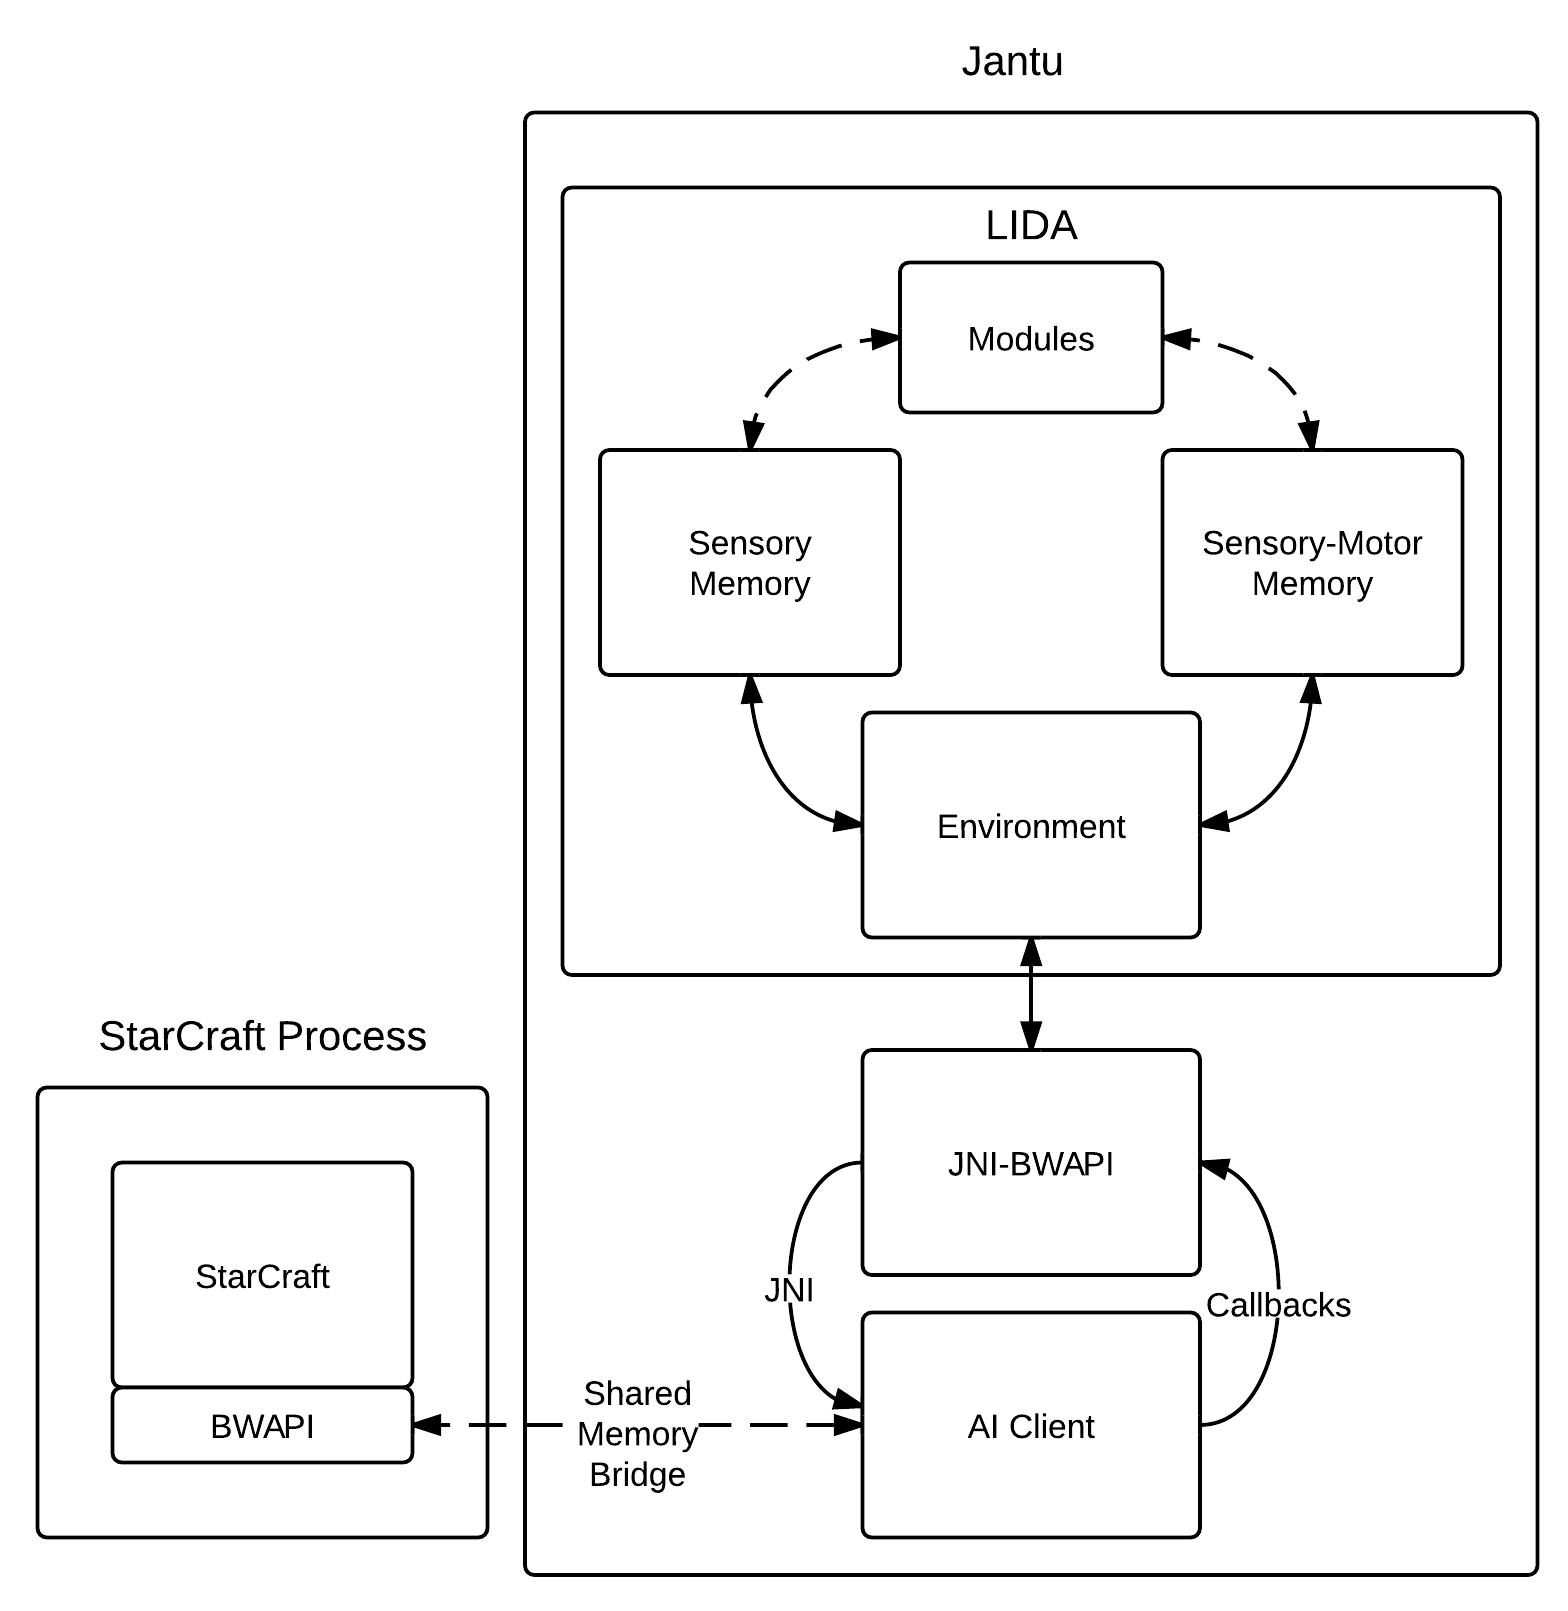
\includegraphics[scale=1.0]{graphics/jantu.png}
\caption{A general architecture overview of Jantu}
\label{fig:jantu}
\end{figure}

Figure \ref{fig:jantu} shows a general overview of the Jantu bots architecture, which consists of 3 main parts. In the Starcraft process the game it self runs together with BWAPI injected into the game client. Since this is all running in c++ and we are using the Java interface for BWAPI our code is run in a separate process that communicates with the Starcraft process using a shared memory bridge, this enables JNI-BWAPI to make calls to BWAPI and retrieve information back across the bridge. 

In the Jantu process JNI-BWAPI is running together with the LIDA framework. In order to integrate the LIDA framework with JNI-BWAPI we setup the framework first with the configurations we needed to get it up and running. This involves describing and structuring the modules you need in different XML configuration files. Also in these files we configure what kind of information that will be possible to use and transmit internally in the LIDA framework. 

JNI-BWAPI consists of different models and types that represent Starcraft information like units and buildings together with a lot of native functions that can be called to communicate with BWAPI. So we integraded this with LIDA by using a custom implementation of the Environment class in LIDA. This class becomes the interface between the domain specific modules of LIDA, the sensory memory and sensory-action memory, and JNI-BWAPI. 

\section{Detectors}
\label{sec:detectors}
Feature detectors is how LIDA perceives it's environment and identifies important aspects of the current game state. They are task that are run at specific intervals and parses the game state at that time in order to identify a given feature that can later be used in different modules in LIDA recognize thoughts and concepts. Each detector usually only identifies one specific feature, but it is possible for one detector to identify several features of they are of the same type. 

These are the detectors we implemented: 
\begin{itemize}
\item \textbf{IdleWorkerFeatureDetector} \\
This feature detector identifies worker units that doesn't have a job, a worker could be gathering resources, constructing buildings or scouting. But for efficiency it should be doing something at all times. 
\item \textbf{LarvaFeatureDetector} \\
This feature detector identifies larvae that are ready to be morphed into units. This is the only way Zerg can create units and when no larvae are available they can't create any more units until more larvae spawn. 
\item \textbf{ResourceFeatureDetector} \\
This feature detector identifies what type of units and buildings that we currently have enough resources available to create. This can be buildings we can construct, units we can morph or upgrades that we can research. 
\item \textbf{SupplyBlockFeatureDetector} \\
This feature detector identifies when we are getting close to being supply blocked, that means that we can't build any more units because another supply-granting building/unit is created.
\item \textbf{UnsaturatedResourcesFeatureDetector} \\
This feature detector identifies whether or not our available resource nodes have are saturated with enough workers that are gathering them. This can be used to decide if we need to build more workers or not.
\end{itemize}

Feature detectors can be created that detect almost every aspect of the game, and they can be everything from simply detecting the existence of specific units or game elements to more complex detectors that detect army compositions or enemy tactics and strategies. The more of them you implement the more advanced concepts you can identify and that opens up more advanced strategies you can perform yourself. 

\section{Action Execution}
\label{sec:actionexecution}
After LIDA has selected a focus of conciseness and an appropriate action has been selected from the behaviour net, the selected action must be executed. This gets execute by having the sensory-motor memory make calls to the environment class that functions as the interface between LIDA and JNI-BWAPI. 

These are the possible action that gets selected and executed in Jantu:
\begin{itemize}
\item \textbf{Mine minerals} \\
This actions takes a worker that is not currently performing a task and orders it to start mining minerals from an unsaturated mineral deposit.
\item \textbf{Build worker} \\
This action takes an available larva and starts the morphing process to make it into a worker drone. 
\item \textbf{Build supply} \\
This action constructs a building or unit that grants increased supply. This can be a building or a unit depending on the race. For Zerg it morphs a drone into an overlord that increases your supply cap. 	
\end{itemize}

How the action is implemented in the sensory-memory is up to the developer, as long as it performs its given function. It can be really simple implementation or you could do something more complex, LIDA is there to decide what parts or game state to focus on, and to make the decision on what action to perform, not how that action is executed.